\section{Data collection and analysis environment overview}
\label{sec3}

The \gls{sanren} was conceptualised in 2003 and implemented by the Meraka Institute of the \gls{csir} under contract to the \gls{dst} from 2008 onwards  \cite{draai2015implementing}. 


The \gls{sanren} network has approximately one million users spread across 151 sites throughout South Africa. The \gls{sanren} has a national backbone capacity of 10 Gbps. Typical client hand off is 1 Gbps though some main campuses connect at 10 Gbps. The average bandwidth per site is 2.82 Gbps. Fig.~\ref{fig:SANREN_net} depicts the high-level network architecture of the \gls{sanren} network  \cite{draai2015implementing}. The \gls{sanren} network has two main connection points to the international Internet infrastructure, namely SEACOM and \gls{wacs} \cite{draai2015implementing}.

\begin{figure}[h]
    \centering
    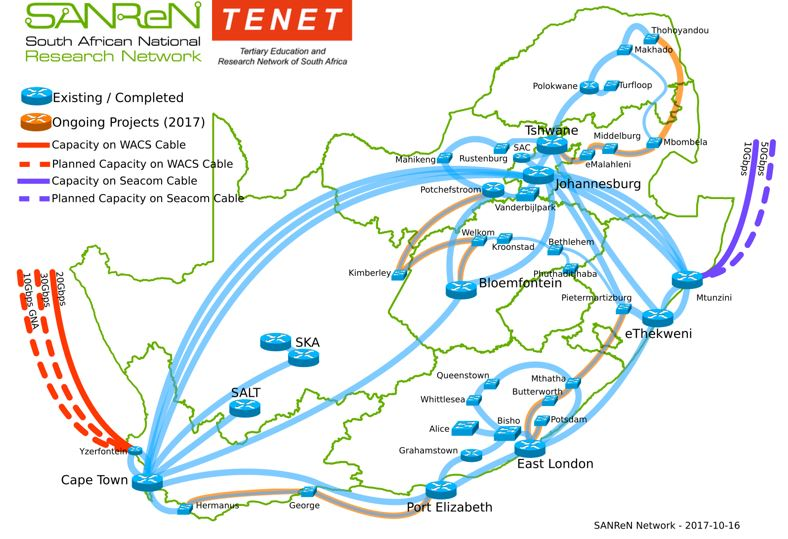
\includegraphics[width=\columnwidth]{section_3/SANREN_Net.JPG}
    \caption{\gls{sanren} network layout \cite{draai2015implementing}}
    \label{fig:SANREN_net}
\end{figure}

The size and scope of the \gls{sanren} infrastructure makes detecting and responding to network attacks challenging. Various sensors have been deployed on the \gls{sanren} to assist with detecting malicious activity.


These sensors include:
\begin{itemize}
    \item Network honeypots -- A honeypot is a closely monitored network decoy   \cite{mokube2007honeypots}. A honeypot can be a virtualised or physical replica of a networked service or infrastructure component. The goal of a honeypot is to act as a distraction for an attacker. A honeypot usually possesses several logging and measurement capabilities to capture the activities performed by the attacker on the decoy  \cite{spitzner2003honeypots2}.
    \item Network telescopes -- A network telescope is an unallocated IP address space which has some form of packet capture mechanism attached to it. Since the IP address space is unallocated, any packet which is routed to the address space is either a broadcast package, misconfigured host, network probe/scans, or potentially a malicious software seeking to spread across the network  \cite{irwin2012network}.
    \item Network flow collectors -- A network flow collector collects the bi-directional meta data of a network connection stream \cite{Graham2017Primer}.
\end{itemize}
For this paper only the network flow collection data is used for analysis due to privacy concerns and data availability. 


The \gls{sanren} \gls{csirt} uses NetFlow v9 (RFC 7011 \cite{RFC7011}) sensors to collect network flow data for traffic analysis and anomaly detection. NetFlow is a data model originally proposed by Cisco in 1996, to capture network flow information  \cite{Graham2017Primer}.  Network flow data is a representative model of the network traffic being transferred over the network. At the bare minimum a flow can be captured as a 6-tuple of information elements: source IP address, destination IP address, source port, destination port, protocol used and time-stamp  \cite{dietz2013passive}. NetFlow v9 does provide the option to add additional data element templates to the data model but for this analysis these additional templates are not required.

The main benefits of using  network flows as a means to detect cyber
incidences over traditional packet capture techniques is the speed at which network flow traffic can be captured. NetFlow is a high speed flow export protocol and thus presents less of a bottle neck for network data collection than traditional packet capture technologies  \cite{hofstede2014flow}.

Another benefit of flow-based data capture over packet capture techniques is the reduced privacy concerns. NetFlow only collects meta data related to the network traffic flow, it does not collect the data packet content \cite{hofstede2014flow}. 

A side effect of only capturing flow meta data is that packet payloads and specific packet signatures can not be detected using NetFlow. Based on the taxonomy of \gls{dos} attacks, presented by Specht \textit{et al.} \cite{specht2004distributed}, network flow analysis is best suited for detecting Bandwidth depletion attacks rather than Resource depletion attacks. Resource depletion attacks tends to exploit weakness with network protocols or inject malicious packet payloads into the network  \cite{specht2004distributed}.

The \gls{sanren} \gls{csirt} collects network flow data from various network exchange points throughout South Africa. The two primary network flow collection points are located at the \gls{wacs} and SEACOM connection points to the SANReN network. The routers at these collection points export all network flow data originating from or destined to the international IP address space, to a centralised NetFlow Collector. On average each of these collection nodes collects 20 Gigabytes of NetFlow data per day. Once the Netflow data has been exported. The flow data is analysed by the \gls{sanren} \gls{csirt} NetFlow Analyser system. If the analysis system detects any abnormal traffic an alert is generated and the \gls{sanren} \gls{csirt} is tasked to investigate the anomaly.

In Section~\ref{sec4} the data collected from these network flow collectors is used to detect the Memcached attack.

